% Nicholas M. Rathmann <rathmann@nbi.ku.dk>

\documentclass[tikz,12pt,border=0pt]{standalone}

\usepackage{pgfplots,physics}
\usepackage{newtxtext,newtxmath} % RSPA-like font

\usetikzlibrary{arrows.meta,calc,backgrounds,decorations.markings}
\usepackage{tikz-3dplot}
\tdplotsetmaincoords{60}{130}
\tdplotsetrotatedcoords{0}{0}{0} 

\usepackage{xcolor}
\definecolor{cice}{HTML}{dcf0fd}
\definecolor{S1}{HTML}{a6dba0} % fast
\definecolor{S1d}{HTML}{1b7837}
\definecolor{S2}{HTML}{c2a5cf} % slow
\definecolor{S2d}{HTML}{762a83}

\tikzset{
	every picture/.style={
		font=\fontsize{21}{21}\selectfont, 
		line width=2pt, 
		background rectangle/.style={iceshading, shading angle=180}, 
		show background rectangle, inner frame xsep=1.5ex, inner frame ysep=3.5ex,	
	},
    iceshading/.style={top color=cice!60, bottom color=gray!5},
	anno/.style={anchor=north,align=center},
	arr/.style={-{Stealth[scale=1.4]}, black},
	annosmall/.style={anchor=north,align=center, font=\fontsize{17}{16}\selectfont,},
    %%% waves
	axis/.style={black, line width=1.5pt, -{Latex[scale=1.2]},	},
    vector/.style={line width=1.5pt}, 
	wavescope/.style={tdplot_main_coords, tdplot_rotated_coords},
	wavy/.style={variable=\t,domain=0:pi/2*\Nhalf,samples=100},
	annowave/.style={anchor=north, rotate=90, font=\fontsize{18.5}{11}\selectfont},
}

\begin{document}

\begin{tikzpicture}[]

%%% Polyclouds

\gdef\scalecloud{0.9}

\node[] (P1) at (0,0) {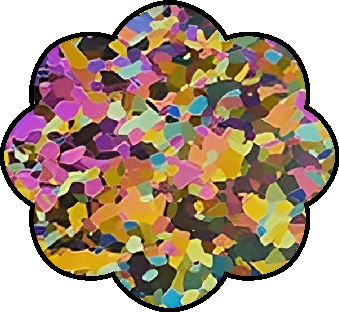
\includegraphics[scale=\scalecloud]{polycloud/thinsection.pdf}};
\node[anno] at (P1.south) {Ice polycrystal};

\node[] (P2) at (6.0cm,0) {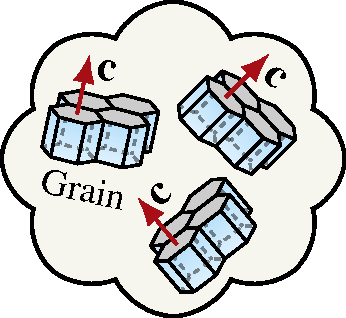
\includegraphics[scale=\scalecloud,page=1]{polycloud/polycrystal.pdf}};
\node[anno] at (P2.south) {Orientation fabric};

%%% c-axis distribution

\node[anchor=north] (P3) at (11.5cm,2.2cm) {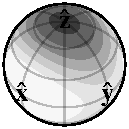
\includegraphics[scale=1.8,page=1]{a2/caxis-distribution.pdf}};
\node[anchor=north, align=center] at ($(P3.south)-(0.1cm,0.36cm)$) {Crystal $c$-axis\\distribution};

%%% a2

\node[anchor=north] (P4) at (16.99cm,2.8cm) {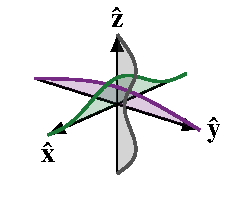
\includegraphics[scale=1.65]{a2/a2.pdf}};
\node[anchor=north,align=center] at ($(P4.south)+(0.4cm,0.7cm)$) {Distribution projected\\ onto principal axes};
\node[annosmall,S1d] (L1) at (19.8cm,0.7cm) {smaller\\ variance};
\node[annosmall,S2d] (L1) at (18.7cm,-0.85cm) {larger\\ variance};

%%% Eigenpolarized waves

\pgfmathsetmacro\A{0.9}
\pgfmathsetmacro\Nhalf{3} % number of half periods to draw
\pgfmathsetmacro\Nvechalf{5} % number of polarization lines per half period
\pgfmathsetmacro\Nvectot{\Nhalf*(\Nvechalf+1)} % total number of polarization lines
\pgfmathsetmacro\wlenf{0.65} % "wave length"
\pgfmathsetmacro\wlens{0.50} % "wave length"

\pgfmathsetmacro\zmax{-pi/2*\Nhalf*\wlenf}
\pgfmathsetmacro\ymax{1.4}
\pgfmathsetmacro\dw{-\A*0.2*0}

\pgfmathsetmacro\zshadow{1.37*\zmax}

\gdef\waveaxis#1#2#3#4#5{
  \draw[axis,black] (0,0,0) -- ++(0,0,1.22*\zmax) node[pos=0.96,#5] {$\vu{k}$};  	
  \draw[axis] (0,0,0) -- ++(0,0,0.9*\ymax) node[black,pos=0.85,right=0.1em] {$\vu{z}$};
  \draw[axis] (0,-0.3*\ymax,0) -- (0,\ymax,0) node[black,pos=0.85,above=0.2em] {$\vu{y}$} node[#1,pos=0.97,below=0.3em,xshift=0.1em] {$#3$};
  \draw[axis] (-0.3*\ymax,0,0) -- (\ymax,0,0) node[black,pos=0.85,above=0.4em] {$\vu{x}$} node[#2,pos=0.98,below=0.4em,xshift=-0.2em] {$#4$};
}

% Fast mode

\gdef\xzero{22.5cm}
\gdef\yzero{1.5cm}
  
\begin{scope}[wavescope, xshift=\xzero, yshift=\yzero]	

	\foreach \k [evaluate={\t=\k*pi/2/(\Nvechalf+1); \angle=\k*90/(\Nvechalf+1);}] 
		in {1,...,\Nvectot}{ \draw[vector,S1]  (0,0,-\t*\wlenf) -- ++({\A*sin(2*\angle)},0,0); }
	
	\waveaxis{black}{S1d}{}{\vu{p}}{left=0.2em, yshift=-0.2em}
	\draw[S1d,wavy] (0,0,-\dw) -- plot ({\A*sin(\t*360/pi)},0,-\t*\wlenf) -- ++(0,0,\dw);
	\draw[S1d,wavy] (-\A,0,\zshadow) -- ++(2*\A,0,0);
\end{scope}

% Slow mode
	
\gdef\dxslower{\xzero+2.7cm}

\begin{scope}[wavescope, xshift=\dxslower, yshift=\yzero]
	
	\foreach \k [evaluate={\t=\k*pi/2/(\Nvechalf+1); \angle=\k*90/(\Nvechalf+1);}] 
		in {1,...,\Nvectot}{ \draw[vector,S2]  (0,0,-\t*\wlens) -- ++(0,{\A*sin(2*\angle)},0); }
	
	\waveaxis{S2d}{black}{\vu{p}}{}{right=0.1em}
	\draw[S2d,wavy] (0,0,-\dw) -- plot (0,{\A*sin(\t*360/pi)},-\t*\wlens) -- ++(0,0,\dw);
	\draw[S2d,wavy] (0,-\A,\zshadow) -- ++(0,2*\A,0);
\end{scope}

% Annotations

\begin{scope}[shift={(\xzero+0.36cm,-0.8cm)}]
	\node[annowave,S1d] at (0,0) {Faster};
	\node[annowave,S2d] at (1.2cm,0) {Slower};
	\node[anchor=north,align=center] at (1cm,-1.75cm) {Eigenpolarized\\ waves};
\end{scope}

%%% Bending arrows

\gdef\arrlen{4em}
\draw[arr] ($(P1.45)-(0.4cm,0.7cm)$) to[bend left=30] ++(\arrlen,0);
\draw[arr] ($(P2.45)-(0.3cm,0.7cm)$) to[bend left=30] ++(\arrlen,0);
\draw[arr] ($(P2.45)-(-5.0cm,0.8cm)$) to[bend left=30] ++(\arrlen,0);

\end{tikzpicture}
\end{document}